\documentclass[12pt]{article}
\usepackage[left = 1in, right = 1in, top = 1in, bottom = 1in]{geometry}
\usepackage{textcomp}
\usepackage{gensymb}
\usepackage{paralist}
\usepackage{cancel}
\usepackage{enumitem}
\usepackage{amsmath}
\usepackage{amssymb}
\usepackage{amsthm}
\usepackage{tkz-euclide}
\usepackage{hyperref}
\usepackage{esdiff}
\usepackage{parskip}
\usepackage{accents}
\usepackage{xcolor}

\usetikzlibrary{arrows.meta,positioning}

\newtheoremstyle{customstyle}
  {8pt} % Space above (adjust as needed)
  {0pt} % Space below (adjust as needed)
  {} % Body font
  {} % Indent amount
  {\bfseries} % Theorem head font
  {. } % Punctuation after theorem head
  {0pt} % Space after theorem head
  {} % Theorem head spec
\theoremstyle{customstyle}
\newtheorem{theorem}{Theorem}[section]
\newtheorem{exercise}{Exercise}[section]
\newtheorem{claim}[theorem]{Claim}
\newtheorem{prop}[theorem]{Proposition}
\newtheorem{corollary}[theorem]{Corollary}
\newtheorem{lemma}[theorem]{Lemma}
\newtheorem{definition}[theorem]{Definition}
\newtheorem{question}{Question}
\newtheorem{subquestion}{Part}[question]

\def\definitionautorefname{Definition}
\def\corollaryautorefname{Corollary}

\newenvironment{nonproof}{\par $\cancel {\text{\textit{Proof}}}.$}{\hfill$\cancel\square$}

\def\contra{\tikz[baseline, x=0.22em, y=0.22em, line width=0.032em]\draw (0,2.83)--(2.83,0) (0.71,3.54)--(3.54,0.71) (0,0.71)--(2.83,3.54) (0.71,0)--(3.54,2.83);}
\newenvironment{answer}{\par\noindent\textit{Answer.}}{\par}

\renewcommand{\CancelColor}{\color{red}}
\renewcommand{\Re}{\operatorname{Re}}
\renewcommand{\Im}{\operatorname{Im}}
\renewcommand{\bar}{\overline}
% \renewcommand{\vec}[1]{\undertilde{\mathrm{#1}}}
% \renewcommand{\vec}[1]{\undertilde{#1}}
% \renewcommand{\vec}[1]{\underline{#1}}
\renewcommand{\vec}[1]{\mathbf{#1}}
\newcommand{\unitvec}[1]{\hat{\vec{#1}}}
\newcommand{\sol}{$\operatorname{sol}^{\simeq}$}
\newcommand{\Arg}{\operatorname{Arg}}
\newcommand{\Log}{\operatorname{Log}}
\newcommand{\vecspan}{\operatorname{span}}
\newcommand{\id}[1]{\operatorname{id}_{#1}}
\newcommand{\indic}[1]{i_{#1}}
\newcommand{\Sym}{\operatorname{Sym}}
\newcommand{\Isom}{\operatorname{Isom}}
\newcommand{\di}{\mathrm{d}}
\newcommand{\gen}[1]{\langle{#1}\rangle}

\definecolor{applegreen}{rgb}{0.55, 0.71, 0.0}
\definecolor{ufogreen}{rgb}{0.24, 0.82, 0.44}


\begin{document}
    \begin{question}
        Let $D$ be the interior of the circle $|z - 1 - i| = 1$.
        Show, by using suitable inequalities for $|z_{1} \pm z_{2}|$,
        that if $z \in D$ then $\sqrt{5} - 1 < |z - 3| < \sqrt{5} + 1$.
    \end{question}

    \begin{answer}
        Since $D$ is the interior, if $z \in D$ we have $|z - (1 + i)| < 1$,
        or $|(z - 3) - (-2 + i)| < 1$, or $|(z - 3) + (2 - i)| < 1$.
        we have
        \begin{align*}
            |z_{1} + z_{2}| &\le |z_{1}| + |z_{2}|\\
            |z_{1} - z_{2}| &\ge |z_{1}| - |z_{2}|
        \end{align*}
        so
        \begin{align*}
            |z_{1}| &\ge |z_{2}| - |z_{1} + z_{2}|\\
            |z_{1}| &\le |z_{2}| + |z_{1} - z_{2}|
        \end{align*}
        For an upper bound, let $z_{1} = z - 3$ and $z_{2} = -2 + i$, then
        \begin{align*}
            |z - 3| &\le |-2 + i| + |z - 3 + 2 - i|\\
                    &= \sqrt{5} + |z - 1 - i|\\
                    &< \sqrt{5} + 1
        \end{align*}
        For a lower bound, let $z_{1} = z - 3$ and $z_{2} = 2 - i$, then
        \begin{align*}
            |z - 3| &\ge |2 - i| - |z - 3 + 2 - i|\\
                    &= \sqrt{5} - |z - 1 - i|\\
                    &> \sqrt{5} - 1
        \end{align*}
        Combining the two yields $\sqrt{5} - 1 < |z - 3| < \sqrt{5} + 1$.
    \end{answer}

    \begin{subquestion}
        Obtain the same result geometrically.
        (start by considering the line through the centre
        of the circle and the point 3)
    \end{subquestion}


    \begin{answer}
        \begin{center}
            \begin{tikzpicture}[scale=3]
                \tkzDefPoint(1,1){A}
                \tkzDefPoint(2,1){A'}
                \tkzDefPoint(3,0){B}
                \tkzInterLC(A,B)(A,A') \tkzGetPoints{C'}{C}

                \tkzInit[xmin=0,ymin=0,xmax=3,ymax=2]
                \tkzDrawX[label=Re]
                \tkzDrawY[label=Im]

                \tkzDrawPoints[fill=black](A,B,C)
                \tkzLabelPoint[left, inner sep=0.4cm, yshift=-0.2cm](A){$1+i$}
                \tkzLabelPoint[below, inner sep=0.3cm, xshift=0.1cm](B){$3$}
                \tkzDrawLine[dashed](B,C')

                \tkzDrawCircle(A,A')
                \tkzDrawSegment[dim={$\sqrt{5}$,-0.5cm,}](A,B)
                % \tkzDrawSegment[dim={$1$,0.5cm,}](A,C)
                \tkzDrawSegment[dim={$\sqrt{5}-1$,0.5cm,}](C,B)
                \tkzDrawSegment[dim={$\sqrt{5}+1$,1.2cm,}](C',B)
            \end{tikzpicture}
        \end{center}
    \end{answer}
    Thus, $\sqrt{5}-1 \le |z-3| \le \sqrt{5}+1$.

    \begin{question}
        Given $|z|=1$ and $\arg z = \theta $, find both
        algebraically and geometrically the modulus-argument
        forms of $1+z$ and $1-z$.
    \end{question}
    \begin{answer}
        We have $z = \cos\theta + i\sin\theta$, so
        \begin{align*}
            1+z 
            &= (1+\cos\theta)+i(\sin\theta)\\
            |1+z|^{2} 
            &= (1+\cos\theta)^{2} + \sin^{2}\theta\\
            &= 1+2\cos\theta+1\\
            |1+z|
            &= \sqrt{2(1+\cos\theta)}
        \end{align*}
        Let $\alpha = \arg(1+z)$, we have
        \begin{align*}
            \cos\alpha 
            &= \frac{1+\cos\theta}{\sqrt{2(1+\cos\theta)}}\\
            &= \sqrt{\frac{1+\cos\theta}{2}}\\
            &= \sqrt{\frac{1+2\cos^{2}(\theta/2)-1}{2}}\\
            \cos\alpha 
            &= |\cos(\theta/2)|
        \end{align*}
        But we have $-\pi<\theta\le\pi$, so $\cos(\theta/2) \ge 0$, and $\cos\alpha=\cos(\theta/2)$.
        Thus, we have $\alpha = \pm\theta/2$, so
        \begin{align*}
            \sin\alpha
            = \pm\sin(\theta/2)
            &= \frac{\sin\theta}{\sqrt{2(1+\cos\theta)}}\\
            \pm &= \frac{\sin\theta}{\sin(\theta/2)\sqrt{2(1+\cos\theta)}}
        \end{align*}
        Since square roots are positive, and $\sin\theta$ and $\sin(\theta/2)$ have the
        same sign, $\pm$ collapses to $+$, and we have $\alpha = \theta/2$.

        Similarly, we have
        \begin{align*}
            1-z
            &= (1-\cos\theta)+i(-\sin\theta)\\
            |1-z|^{2}
            &= (1-\cos\theta)^{2} + \sin^{2}\theta\\
            &= 2(1-\cos\theta)\\
            |1-z|
            &= \sqrt{2(1-\cos\theta)}
        \end{align*}
        Letting $\beta=\arg(1-z)$, we have
        \begin{align*}
            \cos\beta
            &= \frac{1-\cos\theta}{\sqrt{2(1-\cos\theta}}\\
            &= \sqrt{\frac{1-\cos\theta}{2}}\\
            \cos\beta
            &= |\sin(\theta/2)|
        \end{align*}
        To forgo sign issues, let $0\le\phi<2\pi$ such that 
        $\cos\phi=\cos\theta$ and $\sin\phi=\sin\theta$. 
        Note that we have
        \[
        \phi = \begin{cases}
            \theta & \text{if }\theta \ge 0\\
            \theta + 2\pi & \text{if }\theta < 0.\\
        \end{cases}
        \]
        Now we have $\sin(\theta/2) = \sin(\phi/2) \ge 0$, so
        \[
            \cos\beta = \sin(\phi/2) = \cos(\pi/2 - \phi/2),
        \]
        so $\beta=\pm(\pi-\phi)/2$. To determine the sign, we have
        \begin{align*}
            \sin\beta = \pm\sin(\pi/2 - \phi/2) 
            &= \frac{-\sin\theta}{\sqrt{2(1-\cos\theta)}}\\
            \pm
            &= -\frac{\sin\theta}{\cos(\phi/2)\sqrt{2(1-\cos\theta)}}
        \end{align*}
        When $\theta\ge 0$, we have $\phi\le\pi$, so
        $\sin\theta \ge 0$ and $\cos(\phi/2) \ge 0$, so $\pm$ collapses to $-$.
        When $\theta<0$, we have $\phi\ge\pi$, so
        $\sin\theta \le 0$ and $\cos(\phi/2) \le 0$, so $\pm$ collapses again to $-$.
        Thus,
        \begin{align*}
            \beta 
            &= \frac{\phi-\pi}{2}\\
            &= \begin{cases}
                (\theta-\pi)/2 & \text{if }\theta \ge 0\\
                (\theta+\pi)/2 & \text{if }\theta < 0\\
            \end{cases}
        \end{align*}
        Which concludes the algebraic argument.
        Geometrically, we have

        \begin{center}
            \begin{tikzpicture}
                [scale=5, >=stealth,
                angle label/.style={fill=white,circle,inner sep=1pt},
                ]
                \draw[->] (-0.7,0) coordinate (-X)
                    -- (1.6,0) coordinate (X)
                    node[below] {Re};
                \draw[->] (0,-1.2) coordinate (-Y)
                    -- (0,1.2) coordinate (Y)
                    node[left] {Im};

                \draw (0, 0) coordinate (O)
                    ++(70:1) coordinate (Z)
                    ++(1, 0) coordinate (Z1)
                      (70:-1) coordinate (-Z)
                    ++(1, 0) coordinate (Z2);
                
                \draw[->] (O) -- (Z) node[above left] {$z$};
                \draw[->] (Z) -- (Z1) node [above right] {$1+z$};
                \draw[dashed] (O) -- (Z1);

                \tkzMarkAngle[size=0.12cm](X,O,Z)
                \tkzLabelAngle[pos=0.17pt,angle label](X,O,Z) {$\theta$}
                \tkzMarkAngle[size=0.25cm](X,O,Z1)
                \tkzLabelAngle[pos=0.31pt,angle label](X,O,Z1) {$\alpha$}

                \tkzMarkAngle[size=0.15cm,red](Z,Z1,O)
                \tkzLabelAngle[pos=0.21pt,red,angle label](Z,Z1,O) {$\alpha$}
                \tkzMarkAngle[size=0.25cm,red](Z1,O,Z)
                \tkzLabelAngle[pos=0.31pt,red,angle label](Z1,O,Z) {$\alpha$}

                \draw[->] (O) -- (-Z) node[below left] {$-z$};
                \draw[->] (-Z) -- (Z2) node [below right] {$1-z$};
                \draw[dashed] (O) -- (Z2);

                \tkzMarkAngle[size=0.12cm,red](-X,O,-Z)
                \tkzLabelAngle[pos=0.18pt,red,angle label](-X,O,-Z) {$\theta$}
                \tkzMarkAngle[size=0.12cm](Z2,O,X)
                \tkzLabelAngle[pos=0.2pt,angle label](Z2,O,X) {$-\beta$}

                \tkzMarkAngle[size=0.12cm,red](-Z,O,Z2)
                \tkzLabelAngle[pos=0.2pt,red,angle label](-Z,O,Z2) {$-\beta$}
                \tkzMarkAngle[size=0.12cm,red](O,Z2,-Z)
                \tkzLabelAngle[pos=0.2pt,red,angle label](O,Z2,-Z) {$-\beta$}
            \end{tikzpicture}
        \end{center}
        In this above diagram, black angles indicate values
        by definition, and red angles those through angle chasing.
        First, for $1+z$, we follow the following argument:
        \begin{compactenum}[(i)]
        \item Since $(1+z)-(z)=1$ is parallel to the real axis,
            the angle formed by the origin and $z$ around $1+z$ is also $\alpha$.
        \item Since $|z|=1=|(1+z)-(z)|$, the triangle formed by
            the origin, $z$, and $1+z$ is isosceles, so the
            angle formed by $z$ and $1+z$ around the origin is also $\alpha$.
        \item Thus, $\theta = 2\alpha$, so $\alpha = \theta/2$.
        \end{compactenum}
        For $1-z$, the above diagram only shows positive $\theta$. We have the following steps:
        \begin{compactenum}[(i)]
        \item The angle formed by $-z$ and the negative real axis is
            opposite to the angle formed by $z$ and the positive real axis,
            so the former is also $\theta$.
        \item Since $(1-z)-(-z)=1$ is parallel to the real axis,
            the angle formed by the origin and $-z$ around $1-z$ is also $\beta$.
        \item Since $|-z|=1=|(1-z)-(-z)|$, the triangle is isosceles,
            so the angle formed by $-z$ and $1-z$ around the origin is also $\beta$.
        \item Thus, $\theta - 2\beta = \pi$, so $\beta = (\theta-\pi)/2$.
        \end{compactenum}
        The diagram for negative $\theta$ is as follows.
        \begin{center}
            \begin{tikzpicture}
                [scale=5, >=stealth,
                angle label/.style={fill=white,circle,inner sep=1pt},
                ]
                \draw[->] (-0.7,0) coordinate (-X)
                    -- (1.0,0) coordinate (X)
                    node[below] {Re};
                \draw[->] (0,-1.2) coordinate (-Y)
                    -- (0,1.2) coordinate (Y)
                    node[left] {Im};

                \draw (0, 0) coordinate (O)
                      (-70:1) coordinate (Z)
                      (-70:-1) coordinate (-Z)
                    ++(1, 0) coordinate (Z2);
                
                \draw[->] (O) -- (Z) node[below left] {$z$};
                
                \draw[->] (O) -- (-Z) node[above left] {$-z$};
                \draw[->] (-Z) -- (Z2) node [above right] {$1-z$};
                \draw[dashed] (O) -- (Z2);

                \tkzMarkAngle[size=0.12cm](Z,O,X)
                \tkzLabelAngle[pos=0.20pt,angle label](Z,O,X) {$-\theta$}
                \tkzMarkAngle[size=0.12cm](X,O,Z2)
                \tkzLabelAngle[pos=0.18pt,angle label](X,O,Z2) {$\beta$}

                \tkzMarkAngle[size=0.12cm,red](Z2,O,-Z)
                \tkzLabelAngle[pos=0.18pt,red,angle label](Z2,O,-Z) {$\beta$}
                \tkzMarkAngle[size=0.12cm,red](-Z,Z2,O)
                \tkzLabelAngle[pos=0.18pt,red,angle label](-Z,Z2,O) {$\beta$}
            \end{tikzpicture}
        \end{center}
        By the exact same argument, this time we have $2\beta - \theta = \pi$,
        so $\beta = (\theta + \pi)/2$.
        Thus, algebraic and geometric arguments have produced the same answer.
    \end{answer}

    \begin{subquestion}
        Show that the locus of $w$ as $z$ varies with $|z|=1$, where
        \[
        w^{2} = \frac{1-z}{1+z},
        \]
        is a pair of straight lines.
    \end{subquestion}
    \begin{answer}
        Let $\theta = \arg z$, as in last part.
        First, consider the argument, by taking $\arg$ on both sides.
        \begin{align*}
            2\arg w
            &= \arg(1-z) - \arg(1+z)\\
            &= \arg(1-z) - \theta/2
        \end{align*}
        If $\theta \ge 0$, then
        \begin{align*}
            2\arg w
            &= (\theta-\pi)/2 - \theta/2 + 2n\pi\\
            \arg w
            &= -\frac{\pi}{4} + n\pi
        \end{align*}
        for any $n \in \mathbb{Z}$, which produces $\arg w = -\pi/4$ and $\arg w = 3\pi/4$.
        Collectively, this means that $w$ must lie on the line $y = -x$.

        If $\theta < 0$, then we have
        \begin{align*}
            2\arg w
            &= (\theta+\pi)/2 - \theta/2 + 2n\pi\\
            \arg w
            &= \frac{\pi}{4} + n\pi
        \end{align*}
        for any $n \in \mathbb{Z}$, so $\arg w = \pi/4$ or $\arg w = -3\pi/4$
        are both solutions to the equation,
        which means that $w$ must lie on the line $y = x$.

        Now, examine the modulus.
        \begin{align*}
            |w|^{2} 
            &= \frac{|1-z|}{|1+z|}\\
            &= \sqrt{\frac{1-\cos\theta}{1+\cos\theta}}\\
            &= \sqrt{-1-\frac{1}{1+\cos\theta}}
        \end{align*}
        Some consideration of the range of $\cos\theta$ yields that
        $|w|$ can take any positive real value. Thus,
        $w$ forms the entire lines $y=\pm x$.
    \end{answer}

    \begin{question}
        Consider a triangle in the complex plane with vertices at $0$, $z_{1}$ and $z_{2}$.
        Write down an expression for the general point on the median through $z_{1}$,
        and a similar expression for the general point on the median through $z_{2}$.
        Show that the three medians of the triangle are concurrent.
    \end{question}
    \begin{answer}
        The median through $z_{1}$ must go through $z_{1}$ and $z_{2}/2$, so
        \begin{align*}
            z 
            &= (1-\lambda)(z_{1})+\lambda(z_{2}/2)\\
            &= (1-\lambda)z_{1}+(\lambda/2)z_{2}\\
        \end{align*}
        Similarly, the median through $z_{2}$ must go through $z_{2}$ and $z_{1}/2$,
        so $z = (\mu/2)z_{1}+(1-\mu)z_{2}$.

        Now, for concurrency, we also want the third median,
        which is $z = (z_{1}/2 + z_{2}/2)\nu = (\nu/2)z_{1} + (\nu/2)z_{2}$.
        They intersect at the same point iff there
        exists $\lambda,\mu,\nu$ such that
        \[
            (1-\lambda)z_{1}+(\lambda/2)z_{2} 
            = (\mu/2)z_{1}+(1-\mu)z_{2}
            = (\nu/2)z_{1} + (\nu/2)z_{2}
        \]
        By taking $z_{1}=0$ and $z_{2}=0$, we have
        \[
            1-\lambda = \mu/2 = \nu/2 = 1-\mu = \lambda/2
        \]
        So $1-\lambda = \lambda/2$ and $1-\mu=\mu/2$, so $\lambda=\mu=2/3$.
        From there, we have $\nu=\mu=\lambda=2/3$,
        which satisfies all equations, so the three lines are concurrent,
        and they meet at $z_{1}/3 + z_{2}/3$.
    \end{answer}

    \begin{question}
        Express
        \[
            I = \frac{z^{5}-1}{z-1}
        \]
        as a polynomial in $z$.
        By consider the complex fifth roots of unity $\omega$,
        obtain the four factors of $I$ linear in $z$.
        Hence write $I$ as the product of two real quadratic factors.
    \end{question}
    \begin{answer}
        We have that $z^{5}-1 = (z-1)(z^{4}+z^{3}+z^{2}+z+1)$,
        so $I = z^{4}+z^{3}+z^{2}+z+1$.

        Since $I = (z^{5}-1)/(z-1)$, the roots of $z^{5}-1$
        are also the roots of $I$, unless the root is $1$.
        The roots of $z^{5}-1$ are $\exp(2i\pi k/5)$ for $k=\{0,1,2,3,4\}$.
        For $k=0$, the root is $1$, so that is excluded.
        Four roots remain, and $I$ can only have 4 roots,
        so those are the four roots. Thus
        \[
        I = (1 - e^{2i\pi/5})(1 - e^{4i\pi/5})(1 - e^{-2i\pi/5})(1 - e^{-4i\pi/5})
        \]
        For real quadratic factors, notice that some roots are conjugates of others.
        \begin{align*}
            I 
            &= (z - e^{2i\pi/5})(z - e^{-2i\pi/5})(z - e^{4i\pi/5})(z - e^{-4i\pi/5})\\
            &= (z^{2} - (e^{2i\pi/5} + e^{-2i\pi/5})z + 1)(z^{2} - (e^{4i\pi/5} + e^{-4i\pi/5})z + 1)\\
            &= (z^{2} - 2\cos(2\pi/5)z + 1)(z^{2} - 2\cos(4\pi/5)z + 1)
        \end{align*}
    \end{answer}

    \begin{subquestion}
        By considering the term in $z^{2}$ in the identity
        obtained for $I$, show that
        \[
        4\cos\frac{\pi}{5}\sin\frac{\pi}{10}=1.
        \]
    \end{subquestion}
    \begin{proof}
        Using the quadratic factors, we have that
        the term of $z^{2}$ is
        \[
            z^{2} + 4\cos(2\pi/5)\cos(4\pi/5)z^{2} + z^{2} = (2 + 4\cos^{2}(2\pi/5))z^{2}
        \]
        But the term is also $z^{2}$ by the subtraction, so
        \begin{align*}
            2 + 4\cos(2\pi/5)\cos(4\pi/5) &= 1\\
            4\cos(2\pi/5)\cos(4\pi/5) &= -1\\
            4\cos(4\pi/10)\cos(4\pi/5) &= -1\\
            4\sin(\pi/2 - 4\pi/10)\cos(4\pi/5 - \pi) &= 1\\
            4\sin(\pi/10)\cos(\pi/5) &= 1
        \end{align*}
    \end{proof}

    \begin{question}
        Find all complex numbers $z$ that satisfy $\sin z = 2$.
    \end{question}
    \begin{answer}
        \begin{align*}
            \sin z = \frac{1}{2i}(e^{iz} - e^{-iz})
            &= 2\\
            e^{iz} - e^{-iz}
            &= 4i\\
            (e^{iz})^{2} - 1
            &= 4i(e^{iz})\\
            (e^{iz})^{2} - 4i(e^{iz}) - 1
            &= 0
        \end{align*}
        This is a quadratic of $e^{iz}$, and quadratics
        only have two roots even in the complex plane, so
        \begin{align*}
        e^{iz} 
        &= \frac{4i \pm \sqrt{-16 + 4}}{2}\\
        &= \left(2 \pm \sqrt{3}\right)i\\
        \end{align*}
        Taking $\Log$ on both sides, we have
        \begin{align*}
        iz
        &= \log\left(2 \pm \sqrt{3}\right) + i \Arg\left(\left(4 \pm \sqrt{3}\right)i\right)\\
        &= \log\left(2 \pm \sqrt{3}\right) + i\pi\left(2n+\frac{1}{2}\right)\\
        z
        &= \left(2n+\frac{1}{2}\right)\pi-i\log\left(2 \pm \sqrt{3}\right)
        \end{align*}
        for any $n \in \mathbb{Z}$.
    \end{answer}

    \begin{question}
        Let $z,a,b \in \mathbb{C}$ ($a \ne b$)
        correspond to points $P,A,B$ in the Argand diagram.
        Let $C_\lambda$ be the locus of $P$ defined by $|PA|/|PB|=\lambda$
        where $\lambda$ is a fixed positive constant.
        Show that $C_\lambda$ is a circle if $\lambda \ne 1$,
        and find its centre and radius. 
        What happens if $\lambda = 1$?
    \end{question}
    \begin{answer}
        Intuitively, this means that the ratio between
        the distance to $A$ and the distance to $B$ is constant.
        This immediately yields that $\lambda=1$ gives the
        perpendicular bisector.
        For simplication, let an affine transformation
        such that $a \mapsto -1+0i$ and $b \mapsto 1+0i$. 
        Such a function always exists, with
        \[
        z \mapsto \frac{2}{b-a}\left(z - \frac{a+b}{2}\right)
        \]
        From now on we will work under this transformation.
        Then we have
        \[
            \lambda = \left|\frac{z+1}{z-1}\right|.
        \]
        Assume that $z$ does form a circle.
        to find the center, let's have $x \in \mathbb{R}$ a solution to the equation.
        \begin{align*}
            \frac{x+1}{x-1} &= \pm\lambda\\
            (x+1) &= \pm\lambda(x-1)\\
            x+1 &= \pm\lambda x \mp\lambda\\
            (1\mp\lambda)x &= \mp\lambda-1\\
            x &= -\frac{1\pm\lambda}{1\mp\lambda}
        \end{align*}
        The radius is half the difference between
        the two solutions, so
        \begin{align*}
            r
            &= \frac{1}{2}\left|\frac{1+\lambda}{1-\lambda} - \frac{1-\lambda}{1+\lambda}\right|\\
            &= \frac{1}{2}\left|\frac{(1+\lambda)^{2} - (1-\lambda)^{2}}{(1+\lambda)(1-\lambda)}\right|\\
            &= \frac{2\lambda}{|1-\lambda^{2}|}.
        \end{align*}
        This expression is horrible. Let's consider the center instead.
        The center is the average of the two solutions, so
        \begin{align*}
            c
            &= -\frac{1}{2}\left(\frac{1+\lambda}{1-\lambda} + \frac{1-\lambda}{1+\lambda}\right)\\
            &= -\frac{1}{2} \frac{(1+\lambda)^{2} + (1-\lambda)^{2}}{1-\lambda^{2}}\\
            &= -\frac{1+\lambda^{2}}{1-\lambda^{2}}.
        \end{align*}
        This expression is not much better.
        We can notice that 
        the center is on the left when $\lambda<1$
        and on the right when $\lambda>1$.
        We want a function $f$ that maps
        the reals to the positive numbers so that
        $f(0) = 1$, $f(-x) < 1$, and $f(x) > 1$ where $x > 0$. 
        The exponential function happens to satisfy this,
        so let's try $\lambda = \exp(\alpha)$.
        \begin{align*}
            c
            &= -\frac{1+\lambda^{2}}{1-\lambda^{2}}\\
            &= -\frac{1+\exp(2\alpha)}{1-\exp(2\alpha)}\\
            &= -\frac{\exp(-\alpha)+\exp(\alpha)}{\exp(-\alpha)-\exp(\alpha)}\\
            &= \frac{\cosh\alpha}{\sinh\alpha}\\
            r
            &= \frac{2\exp(\alpha)}{|1-\exp(2\alpha)|}\\
            &= \left|\frac{2\exp(\alpha)}{1-\exp(2\alpha)}\right|\\
            &= \left|\frac{2}{\exp(-\alpha)-\exp(\alpha)}\right|\\
            &= \left|\frac{1}{\sinh\alpha}\right|
        \end{align*}
        Clearly, $c$ is an odd function of $\alpha$,
        and inside the absolute value of $r$ is odd too,
        so $r$ is an even function of $\alpha$.
        Now, knowing the centre and radius, we have
        \begin{align*}
        z &= \frac{\cosh\alpha}{\sinh\alpha}
        + \frac{1}{\sinh\alpha}\exp(i\theta)\\
        &= \frac{1}{\sinh\alpha}(\cosh\alpha + \exp(i\theta))\\
        &= \csch\alpha(\cosh\alpha + \exp(i\theta))
        \end{align*}
        Let's substitute this back.
        \begin{align*}
            \left|\frac{\csch\alpha(\cosh\alpha+\exp(i\theta))+1}{\csch\alpha(\cosh\alpha+\exp(i\theta))-1}\right|
            &= \left|\frac{\cosh\alpha+\exp(i\theta)+\sinh\alpha}{\cosh\alpha+\exp(i\theta)-\sinh\alpha}\right|\\
            &= \left|\frac{\exp(\alpha)+\exp(i\theta)}{\exp(-\alpha)+\exp(i\theta)}\right|\\
            &= \left|\frac{e^{\alpha-i\theta}+1}{e^{-\alpha-i\theta}+1}\right|\\
            &= \left|\frac{(e^{\alpha-i\theta}+1)(e^{-\alpha+i\theta}+1)}{|e^{-\alpha-i\theta}+1|^{2}}\right|\\
            &= \left|\frac{2+e^{-\alpha+i\theta}+e^{\alpha-i\theta}}{|e^{-\alpha}e^{-i\theta}+1|^{2}}\right|\\
            &= \left|\frac{2+e^{-\alpha+i\theta}+e^{\alpha-i\theta}}{(e^{-\alpha}\cos\theta+1)^{2}+e^{-2\alpha}\sin^{2}\theta}\right|\\
            &= \left|\frac{2+e^{-\alpha+i\theta}+e^{\alpha-i\theta}}{e^{-2\alpha}\cos\theta+2e^{-\alpha}\cos\theta+1+e^{-2\alpha}\sin^{2}\theta}\right|\\
            &= \left|\frac{2+e^{-\alpha+i\theta}+e^{\alpha-i\theta}}{e^{-2\alpha}+2e^{-\alpha}\cos\theta+1}\right|\\
            &= \left|\frac{2+e^{-(\alpha-i\theta)}+e^{\alpha-i\theta}}{e^{-2\alpha}+e^{-\alpha}(e^{i\theta}+e^{-i\theta})+1}\right|\\
            &= \left|e^{\alpha}\frac{2+e^{-\alpha}e^{i\theta}+e^{\alpha}e^{-i\theta}}{e^{-\alpha}+e^{\alpha}+e^{i\theta}+e^{-i\theta}}\right|\\
            &= \left|e^{\alpha}\frac{2+e^{-\alpha}e^{i\theta}+e^{\alpha}e^{-i\theta}}{e^{-\alpha}+e^{\alpha}+e^{i\theta}+e^{-i\theta}}\right|\\
            &= \left|e^{\alpha}\frac{(e^{\alpha}+e^{i\theta})(e^{-\alpha}+e^{-i\theta})}{(e^{\alpha}+e^{i\theta})+(e^{-\alpha}+e^{-i\theta})}\right|\\
            &= e^{\alpha}\frac{|(e^{\alpha}+e^{i\theta})(e^{-\alpha}+e^{-i\theta})|}{(e^{\alpha}+e^{i\theta})+(e^{-\alpha}+e^{-i\theta})}\\
        \end{align*}
        Let's just examine $|(e^{\alpha}+e^{i\theta})(e^{-\alpha}+e^{-i\theta})|$.
        \begin{align*}
            &|(e^{\alpha}+e^{i\theta})(e^{-\alpha}+e^{-i\theta})|^{2}\\
            &= |2+e^{i\theta-\alpha}+e^{\alpha-i\theta}|^{2}\\
            &= |(2 + e^{\alpha}\cos\theta + e^{-\alpha}\cos\theta) + i(e^{-\alpha}\sin\theta - e^{\alpha}\sin\theta)|\\
            &= (2 + \cos\theta(e^{\alpha} + e^{-\alpha}))^{2} + \sin^{2}\theta(e^{-\alpha} - e^{\alpha})^{2}\\
            &= 4 + 4\cos\theta(e^{\alpha}+e^{-\alpha}) + \cos^{2}\theta(e^{\alpha} + e^{-\alpha})^{2} + \sin^{2}\theta(e^{-\alpha} - e^{\alpha})^{2}\\
            &= 4 + 2(e^{i\theta}+e^{-i\theta})(e^{\alpha}+e^{-\alpha}) + \cos^{2}\theta(e^{2\alpha} + 2 + e^{-2\alpha}) + \sin^{2}\theta(e^{-2\alpha} - 2 + e^{2\alpha})\\
            &= 2 + 2(e^{i\theta}+e^{-i\theta})(e^{\alpha}+e^{-\alpha}) + 2\cos^{2}\theta - 2\sin^{2}\theta + e^{2\alpha} + 2 + e^{-2\alpha}\\
            &= 2(e^{i\theta}+e^{-i\theta})(e^{\alpha}+e^{-\alpha}) + 2 + 2\cos(2\theta) + (e^{\alpha} + e^{-\alpha})^{2}\\
            &= 2 + (e^{2i\theta} + e^{-2i\theta}) + 2(e^{i\theta}+e^{-i\theta})(e^{\alpha}+e^{-\alpha}) + (e^{\alpha} + e^{-\alpha})^{2}\\
            &= (e^{i\theta} + e^{-i\theta})^{2} + 2(e^{i\theta}+e^{-i\theta})(e^{\alpha}+e^{-\alpha}) + (e^{\alpha} + e^{-\alpha})^{2}\\
            &= \biggl((e^{i\theta} + e^{-i\theta}) + (e^{\alpha} + e^{-\alpha})\biggr)^{2}
        \end{align*}
        Thus, we have
        \begin{align*}
            \left|\frac{\csch\alpha(\cosh\alpha+\exp(i\theta))+1}{\csch\alpha(\cosh\alpha+\exp(i\theta))-1}\right|
            &= e^{\alpha}\frac{|(e^{\alpha}+e^{i\theta})(e^{-\alpha}+e^{-\theta})|}{(e^{\alpha}+e^{i\theta})+(e^{-\alpha}+e^{-i\theta})}\\
            &= e^{\alpha} = \lambda.
        \end{align*}
        Thus, $z=\csch\alpha(\cosh\alpha+\exp(i\theta))$ is a solution
        to the equation, and the locus of that
        is a circle with center at $\coth\alpha$ and radius $\csch\alpha$.

        Without $\alpha$, this can be written
        \[
        z = \frac{1}{\lambda-\lambda^{-1}}(\lambda+\lambda^{-1}+2e^{i\theta})
         = \frac{\lambda^{2}+1+2\lambda e^{i\theta}}{\lambda^{2}-1}
         \]
         With center $\dfrac{\lambda^{2}+1}{\lambda^{2}-1}$ and
         radius $\dfrac{2\lambda}{|\lambda^{2}-1|}$.
    \end{answer}

    \begin{subquestion}
        For the case $a = -b = p$, $p \in \mathbb{R}$ and for each fixed $\mu\in\mathbb{R}$,
        show that
        \[
        S_\mu = \{z \in \mathbb{C} : |z - i\mu| = \sqrt{p^{2} + \mu^{2}}\}
        \]
        is a circle passing through $A$ and $B$ with its centre on the
        perpendicular bisector of $AB$.
    \end{subquestion}
    \begin{answer}
        We apply the transformation again,
        but this time it's simpler, taking the form of $z \mapsto -p^{-1}z$.
        Thus, $a=p=-1$, $b=1$.
        The points on $S_\mu$ thus satisfy
        \[
        |z - i\mu| = \sqrt{1 + \mu^{2}}
        \]
        The perpendicular bisector of AB is the line $x=0$ which
        is defined by $i\mu$ exactly. Substituting $a$ and $b$ gives
        \[
            |\pm 1 - i\mu|^{2}
            = (\pm 1)^{2} + \mu^{2}
            = 1 + \mu^{2}
        \]
        So $A,B$ do lie on the circle.
    \end{answer}

    \begin{subquestion}
        Show that the circles $C_\lambda$ and $S_\mu$
        intersect orthogonally for all $\lambda$, $\mu$.
    \end{subquestion}
    \begin{proof}
        We have $C_\lambda$ as 
        \begin{align*}
            z 
            &= \frac{\lambda^{2}+1+2\lambda e^{i\theta}}{\lambda^{2}-1}.\\
            \left|z - \frac{\lambda^{2}+1}{\lambda^{2}-1}\right|
            &= \frac{2\lambda}{|\lambda^{2}-1|}
        \end{align*}
        Rewriting $S_\mu$ into a similar forms, we have
        \begin{align*}
            z 
            &= i\mu + \sqrt{1+\mu^{2}}e^{i\theta}\\
            |z - i\mu|
            &= \sqrt{1+\mu^{2}}
        \end{align*}
        If two circles intersect orthogonally, we have
        \begin{center}
            \begin{tikzpicture}
                % \clip (-3.5, 0.5) rectangle +(9,5);
                \begin{scope}[rotate=30]
                    \coordinate (O) at (0,0);
                    \coordinate (A) at (4,0);
                    \coordinate (B) at (0,3);
                    \coordinate (C) at (4,3);
                    
                    \draw (A) circle[radius=3] node[below] {$A$};
                    \draw (B) circle[radius=4] node[below] {$B$};
                    \draw (C) node[above, inner sep=0.3cm] {C};

                    \tkzDrawPoints[fill=black](A,B,C)
                    \tkzDrawSegments(A,B B,C C,A)
                    \tkzMarkRightAngle(B,C,A)
                \end{scope}
            \end{tikzpicture}
        \end{center}
        Thus, it suffices to show that $\abs{c_{1}-c_{2}}^{2} = r_{1}^{2} + r_{2}^{2}$.
        In this case, we have
        \begin{align*}
            \text{LHS} 
            &= \abs{\frac{\lambda^{2}+1}{\lambda^{2}-1}-i\mu}^{2}\\
            &= \left(\frac{\lambda^{2}+1}{\lambda^{2}-1}\right)^{2}+\mu^{2}\\
            &= \frac{(\lambda^{2}+1)^{2}}{(\lambda^{2}-1)^{2}}+\mu^{2}\\
            &= \frac{\lambda^{4}+2\lambda^{2}+1}{(\lambda^{2}-1)^{2}}+\mu^{2}\\
            \text{RHS}
            &= \frac{4\lambda^{2}}{(\lambda^{2}-1)^{2}}+1+\mu^{2}\\
            &= \frac{4\lambda^{2}}{(\lambda^{2}-1)^{2}}+1+\mu^{2}\\
            &= \frac{4\lambda^{2}+(\lambda^{2}-1)^{2}}{(\lambda^{2}-1)^{2}}+\mu^{2}\\
            &= \frac{4\lambda^{2}+\lambda^{4}-2\lambda^{2}-1}{(\lambda^{2}-1)^{2}}+\mu^{2}\\
            &= \frac{\lambda^{4}+2\lambda^{2}-1}{(\lambda^{2}-1)^{2}}+\mu^{2} = \text{LHS}
        \end{align*}
    \end{proof}

    \begin{question}
        Show by vector methods that the altitudes of a triangle are concurrent.
    \end{question}
    \begin{proof}
        Let $\triangle ABC$ and $\vec{a},\vec{b},\vec{c}$ be the
        position vectors of $A,B,C$ respectively.
        The altitude from $A$ has $(\vec{r} - \vec{a}) \cdot (\vec{b} - \vec{c}) = 0$,
        so
        \[
        \vec{r} \cdot (\vec{b} - \vec{c}) = \vec{a} \cdot (\vec{b} - \vec{c}).
        \]
        Similarly, $\vec{r}\cdot(\vec{a}-\vec{c}) = \vec{b}\cdot(\vec{a}-\vec{c})$ is
        the altitude from $B$.
        Note that these are actually planes, but in 2D planes are lines.
        Now, if the three altitudes are concurrent,
        then any $\vec{r}$ that satisifes the above two equations should
        also lie on the third altitude, i.e. $(\vec{r} - \vec{c}) \cdot (\vec{a} - \vec{b}) = 0$.
        Thus, let's consider the LHS of that equation.
        \begin{align*}
            (\vec{r}-\vec{c})\cdot(\vec{a}-\vec{b})
            &= \vec{r}\cdot(\vec{a}-\vec{b}) + \vec{c}(\vec{b}-\vec{a})\\
            &= \vec{r}\cdot(\vec{a}-\vec{c}-(\vec{b}-\vec{c}))+\vec{c}\cdot\vec{b}-\vec{c}\cdot\vec{a}\\
            &= \vec{r}\cdot(\vec{a}-\vec{c})-\vec{r}\cdot(\vec{b}-\vec{c})
            +(\vec{c}-\vec{a})\cdot\vec{b}-(\vec{c}-\vec{b})\cdot\vec{a}\\
            &= \vec{b}\cdot(\vec{a}-\vec{c})-\vec{a}\cdot(\vec{b}-\vec{c})
            +(\vec{c}-\vec{a})\cdot\vec{b}-(\vec{c}-\vec{b})\cdot\vec{a}\\
            &= 0
        \end{align*}
        Thus, any intersection of the altitudes of $A$ and $B$ also lie
        on the altitude of $C$, so the three altitudes are concurrent.
    \end{proof}

    \begin{question}
        In three dimensions, the vectors $\vec{x},\vec{y}$ and $\vec{a}$ satisfy
        \[
        \vec{x} + \vec{y}(\vec{x}\cdot\vec{y}) = \vec{a}
        \]
        Show that
        \[
            (\vec{x}\cdot\vec{y})^{2} = \frac{|\vec{a}|^{2}-|\vec{x}|^{2}}{2+|\vec{y}|^{2}}
        \]
    \end{question}
    \begin{proof}
        Assume $\vec{x},\vec{y},\vec{a}$ that satisfy the first equation, then
        \begin{align*}
            \frac{\abs{\vec{a}}^{2}-\abs{\vec{x}}^{2}}{2+\abs{\vec{y}}^{2}}
            &= \frac{\abs{\vec{x}+\vec{y}(\vec{x}\cdot\vec{y})}^{2}-\abs{\vec{x}}^{2}}{2+\abs{\vec{y}}^{2}}\\
            &= \frac{(\vec{x}+\vec{y}(\vec{x}\cdot\vec{y}))(\vec{x}+\vec{y}(\vec{x}\cdot\vec{y}))-\vec{x}\cdot\vec{x}}
            {2+\vec{y}\cdot\vec{y}}\\
            &= \frac{\abs{\vec{x}}^{2}+2(\vec{x}\cdot\vec{y})^{2}+(\vec{x}\cdot\vec{y})^{2}\abs{\vec{y}}^{2}-\vec{x}\cdot\vec{x}}
            {2+\vec{y}\cdot\vec{y}}\\
            &= \frac{(\vec{x}\cdot\vec{y})^{2}(2+\abs{\vec{y}}^{2})}
            {2+\abs{\vec{y}}^{2}}\\
            &= (\vec{x}\cdot\vec{y})^{2}
        \end{align*}
    \end{proof}

    \begin{subquestion}
        Use an inequality involving $\vec{x}\cdot\vec{y}$ and the
        lengths of $\vec{x}$ and $\vec{y}$ to deduce that
        \[
        \abs{\vec{x}}(1+\abs{\vec{y}}^{2}) \ge \abs{\vec{a}} \ge \abs{\vec{x}}
        \]
        Explain the circumstances in which either of the inequalities
        above become equalities, and describe the relation between
        $\vec{x},\vec{y}$ and $\vec{a}$ in these circumstances.
    \end{subquestion}
    \begin{answer}
        \begin{align*}
            \abs{\vec{a}}^{2} 
            &= \vec{a}\cdot\vec{a}\\
            &= (\vec{x}+\vec{y}(\vec{x}\cdot\vec{y}))\cdot(\vec{x}+\vec{y}(\vec{x}\cdot\vec{y}))\\
            &= \abs{\vec{x}}^{2}
            + 2\vec{x}\cdot(\vec{y}(\vec{x}\cdot\vec{y})) 
            + \abs{\vec{y}(\vec{x}\cdot\vec{y})}^{2}\\
            &= \abs{\vec{x}}^{2} 
            + 2(\vec{x}\cdot\vec{y})^{2}
            + (\vec{x}\cdot\vec{y})^{2}\abs{\vec{y}}^{2}\\
            &= \abs{\vec{x}}^{2} + (\vec{x}\cdot\vec{y})^{2}(2 + \abs{\vec{y}}^{2})\\
            &\ge \abs{\vec{x}}^{2}
        \end{align*}
        And since $\abs{\vec{x}}$ and $\abs{\vec{a}}$ are both positive,
        we can take square root on both sides for $\abs{\vec{a}} \ge \abs{\vec{x}}$.
        Equality then occurs when $\vec{x}\cdot\vec{y} = 0$, so if $\vec{x}$ and $\vec{y}$
        are orthogonal. Then, $\vec{a}=\vec{x}$. We have

        We let $\theta$ be the angle between $\vec{x}$ and $\vec{y}$, then
        \begin{align*}
            \abs{\vec{a}}
            &= \abs{\vec{x} + \vec{y}(\vec{x}\cdot\vec{y})}\\
            &\le \abs{\vec{x}} + \abs{\vec{y}(\vec{x}\cdot\vec{y})}\\
            &= \abs{\vec{x}} + \abs{\vec{x}\cdot\vec{y}}\abs{\vec{y}}\\
            &= \abs{\vec{x}} + \abs{\vec{x}}\abs{\vec{y}}^{2}\abs{\cos\theta}\\
            &\le \abs{\vec{x}} + \abs{\vec{x}}\abs{\vec{y}}^{2}\\ 
            &= \abs{\vec{x}}(1 + \abs{\vec{y}}^{2})
        \end{align*}
        In this case, the equality holds when the
        triangle inequality between $\vec{x}$ and $\vec{y}(\vec{x}\cdot\vec{y})$
        has equality, and $\cos\theta = \pm 1$. The criteria
        for both of these things is that $\vec{x}$ is parallel to $\vec{y}$.
        Then $\vec{a}=\vec{x}(1+\abs{\vec{y}}^{2})$.
    \end{answer}

    \begin{question}
        In $\triangle ABC$, let $\vecof{AB} = \vec{u}$, $\vecof{BC} = \vec{v}$ and $\vecof{CA} = \vec{w}$.
        Show that
        \[
        \vec{u}\times\vec{v}=\vec{v}\times\vec{w}=\vec{w}\times\vec{u}
        \]
        and hence obtain the sine rule for $\triangle ABC$.
    \end{question}
    \begin{answer}
        If we take position vectors $\vec{a},\vec{b},\vec{c}$
        for $A,B$ and $C$,
        then we have $\vec{u} = \vec{a} - \vec{b}$,
        $\vec{v} = \vec{b} - \vec{c}$ and $\vec{w} = \vec{c} - \vec{a}$.
        Then,
        \begin{align*}
            \vec{u}\times\vec{v}
            &= (\vec{a}-\vec{b})\times(\vec{b}-\vec{c})\\
            &= \vec{a}\times\vec{b}-\vec{a}\times\vec{c}
            -\vec{b}\times\vec{b}+\vec{b}\times\vec{c}\\
            &= \vec{a}\times\vec{b}-\vec{a}\times\vec{c}+\vec{b}\times\vec{c}\\
            &= \vec{a}\times\vec{b}+\vec{b}\times\vec{c}+\vec{c}\times\vec{a},
        \end{align*}
        noting that $\vec{b}\times\vec{b}=\vec{0}$ and $\vec{a}\times\vec{c} = -\vec{c}\times\vec{a}$.
        Under a cyclic permutation 
        $\vec{a},\vec{b},\vec{c} \mapsto \vec{b},\vec{c},\vec{a}$,
        we have $\vec{u},\vec{v},\vec{w}\mapsto\vec{v},\vec{w},\vec{u}$.
        However, the final expression is invariant under such
        cyclic permutation, so $\vec{u}\times\vec{v}=\vec{v}\times\vec{w}=\vec{w}\times\vec{u}$.

        For the sine rule, we take length on all three sides, 
        and let the angles in the triangle at $A,B,C$ be $\alpha,\beta,\gamma$ so
        \[
            \abs{\vec{u}}\abs{\vec{v}}\sin\beta = \abs{\vec{v}}\abs{\vec{w}}\sin\gamma
            = \abs{\vec{w}}\abs{\vec{u}}\sin\alpha
        \]
        Dividing by $\abs{\vec{u}}\abs{\vec{v}}\abs{\vec{w}}$ we have
        \[
            \frac{\sin\beta}{\abs{\vec{w}}} = \frac{\sin\gamma}{\abs{\vec{u}}}
            = \frac{\sin\alpha}{\abs{\vec{v}}}
        \]
        Thus letting $a,b,c$ be the lengths of the sides opposing $A,B,C$, we have
        \[
            \frac{\sin\beta}{b} = \frac{\sin\gamma}{c}
            = \frac{\sin\alpha}{a}
        \]
        which is the sine rule.
    \end{answer}

    \begin{subquestion}
        Given any three vectors $\vec{p},\vec{q},\vec{r}$ such that
        \[
        \vec{p}\times\vec{q} = \vec{q}\times\vec{r} = \vec{r}\times\vec{p}
        \]
        and $\abs{\vec{p}\times\vec{q}} \ne 0$, show that
        \[
        \vec{p}+\vec{q}+\vec{r}=0
        \]
    \end{subquestion}
    \begin{proof}
        We have that
        \begin{align*}
            \vec{p}\times\vec{q} &= \vec{q}\times\vec{r}\\
            -\vec{q}\times\vec{p} &= \vec{q}\times\vec{r}\\
            \vec{0} &= \vec{q}\times(\vec{p}+\vec{r})\\
            &= \vec{q}\times(\vec{p}+\vec{r})+\vec{q}\times\vec{q}\\
            \vec{0} &= \vec{q}\times(\vec{p}+\vec{q}+\vec{r}).
        \end{align*}
        This implies that $\vec{p}+\vec{q}+\vec{r}$ is 
        parallel to $\vec{q}$. It is trivial to check that this works after
        a cyclic permutation, so $\vec{p}+\vec{q}+\vec{r}$ is also
        parallel to $\vec{p}$ and $\vec{r}$.
        However, since $\abs{\vec{p}\times\vec{q}}\ne 0$, 
        $\vec{p}$ must not be parallel to $\vec{q}$.
        If $\vec{p}+\vec{q}+\vec{r}\ne 0$, this violates the transitivity of being parallel,
        which is a contradiction.
        Thus, $\vec{p}+\vec{q}+\vec{r}=0$.
    \end{proof}

    \begin{question}
        Interpret geometrically the equations
        \begin{equation}
        \vec{r} = (1-\lambda)\vec{a}+\lambda\vec{b}
        \end{equation}
        and
        \begin{equation}
        \vec{r} = (1-\lambda-\mu)\vec{a}+\lambda\vec{b}+\mu\vec{c}
        \end{equation}
        where $\vec{a},\vec{b}$ and $\vec{c}$ are 
        position vectors of points in three dimensions
        and $\lambda,\mu$ are scalar parameters
        that take any real values.
        For each equation, obtain an equivalent
        form that does not involve parameters
        $\lambda$ or $\mu$.
    \end{question}
    \begin{answer}
        Equation (1) represents a line through $\vec{a}$ and $\vec{b}$.
        \begin{align*}
            \vec{r} 
            &= (1-\lambda)\vec{a}+\lambda\vec{b}\\
            &= \vec{a} + \lambda(\vec{b}-\vec{a}).
        \end{align*}
        In programming (especially graphics)
        this is called lerp, short for linear interpolation.
        It has the property that if $0\le\lambda\le1$,
        then it yields the line segment between $\vec{a}$ and $\vec{b}$,
        and $\vec{r}=\vec{a}$ if $\lambda=0$ and $\vec{r}=\vec{b}$ if $\lambda=1$.

        We can rewrite it as $(\vec{r}-\vec{a})\times(\vec{b}-\vec{a}) = 0$,
        the standard equation of a line.

        Similarly, equation (2) seems to represent
        a plane through $\vec{a},\vec{b}$ and $\vec{c}$, since
        \begin{align*}
            \vec{r} 
            &= (1-\lambda-\mu)\vec{a}+\lambda\vec{b}+\mu\vec{c}\\
            &= \vec{a} + \lambda(\vec{b}-\vec{a})+\mu(\vec{c}-\vec{a}).
        \end{align*}
        Thus, we can rewrite this using the standard plane formula
        to get $(\vec{r}-\vec{a})\cdot((\vec{b}-\vec{a})\times(\vec{c}-\vec{a}))=0$.

        When the $\vec{a},\vec{b}$ and $\vec{c}$ are exchanged,
        the locus of $\vec{r}$ in either case never changes.
        However, the parameters do change.
        The following can happen:
        \begin{enumerate}[label=(\roman*)]
        \item If $\vec{a}$ and $\vec{b}$ are exchanged for equation (1),
            the value of the parameter corresponding to any given point
            on the line undergoes $\lambda \mapsto 1-\lambda$.
            This is obvious either geometrically or looking at the equation.
            It can also be interpretted as the line flipping
            around $(\vec{a}+\vec{b})/2$.
        \item If $\vec{b}$ and $\vec{c}$ are exchanged for equation (2),
            the parameters flip, as obvious through the equation.
            Geometrically, the plane flips around the line passing through
            $\vec{a}$ and $(\vec{b}+\vec{c})/2$.
        \item If $\vec{a}$ and $\vec{b}$ are exchanged for equation (2),
            $\lambda \mapsto 1-\lambda$.
            Geometrically, the plane flips around the line passing through
            $\vec{b}$ and $(\vec{a}+\vec{c})/2$.
        \item Similarly, if $\vec{a}$ and $\vec{c}$ are exchanged for equation (2),
            $\mu \mapsto 1-\mu$.
            Geometrically, the plane flips around the line passing through
            $\vec{c}$ and $(\vec{a}+\vec{b})/2$.
        \end{enumerate}
    \end{answer}

    \begin{question}
        Using the identity 
        $\vec{a}\times(\vec{b}\times\vec{c}) 
        = (\vec{a}\cdot\vec{c})\vec{b}-(\vec{a}\cdot\vec{b})\vec{c}$,
        show that
        \begin{compactenum}[(i)]
        \item $(\vec{a}\times\vec{b})\cdot(\vec{c}\times\vec{d})
            = (\vec{a}\cdot\vec{c})(\vec{b}\cdot\vec{d})
            -(\vec{a}\cdot\vec{d})(\vec{b}\cdot\vec{c})$
        \item $\vec{a}\times(\vec{b}\times\vec{c})
            + \vec{b}\times(\vec{c}\times\vec{a})
            + \vec{c}\times(\vec{a}\times\vec{b})
            = 0$
        \end{compactenum}
    \end{question}
    \begin{proof}[Proof of (i)]
        \begin{align*}
            \text{RHS} 
            &= (\vec{a}\cdot\vec{c})(\vec{b}\cdot\vec{d})
            -(\vec{a}\cdot\vec{d})(\vec{b}\cdot\vec{c})\\
            &= \vec{a}\cdot((\vec{b}\cdot\vec{d})\vec{c} - (\vec{b}\cdot\vec{c})\vec{d})\\
            &= \vec{a}\cdot(\vec{b}\times(\vec{c}\times\vec{d}))
        \end{align*}
        This is a scalar triple product, which is invariant under cyclic permutation.
        \begin{align*}
            \text{RHS}
            &= \vec{a}\cdot(\vec{b}\times(\vec{c}\times\vec{d}))\\
            &= (\vec{c}\times\vec{d})\cdot(\vec{a}\times\vec{b})\\
            &= (\vec{a}\times\vec{b})\cdot(\vec{c}\times\vec{d}) = \text{LHS}\\
        \end{align*}
    \end{proof}

    \begin{proof}[Proof of (ii)]
        \begin{align*}
            \text{LHS}\\
            &= \vec{a}\times(\vec{b}\times\vec{c})
            + \vec{b}\times(\vec{c}\times\vec{a})
            + \vec{c}\times(\vec{a}\times\vec{b})\\
            &=
            (\mathcolor{red}{(\vec{a}\cdot\vec{c})\vec{b}}
            - \mathcolor{blue}{(\vec{a}\cdot\vec{b})\vec{c}})
            + (\mathcolor{blue}{(\vec{b}\cdot\vec{a})\vec{c}}
            - \mathcolor{ufogreen}{(\vec{b}\cdot\vec{c})\vec{a}})
            + (\mathcolor{ufogreen}{(\vec{c}\cdot\vec{b})\vec{a}}
            - \mathcolor{red}{(\vec{c}\cdot\vec{a})\vec{b}})\\
            &= 0 = \text{RHS}
        \end{align*}
    \end{proof}

    \begin{subquestion}
        Relate the case when $\vec{c}=\vec{a}$ and $\vec{d}=\vec{b}$ in (i)
        to a well-known trigonometric identity.
    \end{subquestion}
    \begin{answer}
        We have then 
        \begin{align*}
            (\vec{a}\times\vec{b})\cdot(\vec{a}\times\vec{b})
            &= \abs{\vec{a}\times\vec{b}}^{2}\\
            &= \abs{\vec{a}}^{2}\abs{\vec{b}}^{2}\sin^{2}\theta\\
            (\vec{a}\times\vec{b})\cdot(\vec{a}\times\vec{b})
            &= (\vec{a}\cdot\vec{a})(\vec{b}\cdot\vec{b})
            - (\vec{a}\cdot\vec{b})(\vec{b}\cdot\vec{a})\\
            &= \abs{\vec{a}}^{2}\abs{\vec{b}}^{2}(1 - \cos^{2}\theta)
        \end{align*}
        Thus, if $\vec{a} \ne \vec{0}$ and $\vec{b} \ne \vec{0}$, we have
        \begin{align*}
            \sin^{2}\theta &= 1 - \cos^{2}\theta\\
            \sin^{2}\theta + \cos^{2}\theta &= 1
        \end{align*}
    \end{answer}

    \begin{subquestion}
        Evaluate $(\vec{a}\times\vec{b})\times(\vec{c}\times\vec{d})$
        in two ways and compare the results to find
        an explicit linear combination of the four $\vec{a},\vec{b},\vec{c},\vec{d}$ that is zero.
    \end{subquestion}
    \begin{answer}
        We have
        \begin{align*}
            (\vec{a}\times\vec{b})\times(\vec{c}\times\vec{d})
            &= ((\vec{a}\times\vec{b})\cdot\vec{d})\vec{c}
            - ((\vec{a}\times\vec{b})\cdot\vec{c})\vec{d}\\
            -(\vec{c}\times\vec{d})\times(\vec{a}\times\vec{b})
            &= ((\vec{c}\times\vec{d})\cdot\vec{a})\vec{b}
            - ((\vec{c}\times\vec{d})\cdot\vec{b})\vec{a}.
        \end{align*}
        Thus,
        \[
            ((\vec{c}\times\vec{d})\cdot\vec{b})\vec{a}
            - ((\vec{c}\times\vec{d})\cdot\vec{a})\vec{b}
            + ((\vec{a}\times\vec{b})\cdot\vec{d})\vec{c}
            - ((\vec{a}\times\vec{b})\cdot\vec{c})\vec{d} = 0
        \]
    \end{answer}

    \begin{subquestion}
        Given that $[\vec{a},\vec{b},\vec{c}] \equiv \vec{a}\cdot(\vec{b}\times\vec{c})$, show that
        \[
            [\vec{a}\times\vec{b},\vec{b}\times\vec{c},\vec{c}\times\vec{a}]
            = [\vec{a},\vec{b},\vec{c}]^{2}
        \]
    \end{subquestion}
    \begin{proof}
        We assume that the invariance of $[\vec{a},\vec{b},\vec{c}]$
        under cyclic permutation is known. Then
        \begin{align*}
            \text{LHS}
            &=[\vec{a}\times\vec{b},\vec{b}\times\vec{c},\vec{c}\times\vec{a}]\\
            &= (\vec{a}\times\vec{b})\cdot((\vec{b}\times\vec{c})\times(\vec{c}\times\vec{a}))\\
            &= (\vec{a}\times\vec{b})\cdot(
                ((\vec{b}\times\vec{c})\cdot\vec{a})\vec{c}
                - ((\vec{b}\times\vec{c})\cdot\vec{c})\vec{a}
            )\\
            &= (\vec{a}\times\vec{b})\cdot((\vec{a}\cdot(\vec{b}\times\vec{c}))\vec{c})\\
            &= [\vec{a},\vec{b},\vec{c}]((\vec{a}\times\vec{b})\cdot\vec{c})\\
            &= [\vec{a},\vec{b},\vec{c}][\vec{c},\vec{a},\vec{b}]\\
            &= [\vec{a},\vec{b},\vec{c}]^{2} = \text{RHS}
        \end{align*}
    \end{proof}

    \begin{question}
        Let $\vec{a},\vec{b},\vec{c},\vec{d}$ be fixed vectors in three-dimensions.
        For each of the following equations, find all solutions for $\vec{r}$:
        \begin{compactenum}[(i)]
        \item $\vec{r} + \vec{r}\times\vec{d} = \vec{c}$
        \item $\vec{r} + (\vec{r}\cdot\vec{a})\vec{b} = \vec{c}$
        \end{compactenum}
        [In part (ii), consider separately the cases $\vec{a}\cdot\vec{b} \ne -1$
        and $\vec{a}\cdot\vec{b} = -1$.]
    \end{question}
    \begin{answer}
        (i)
        We have, after rearranging, that $\vec{r}\times\vec{d} = \vec{c}-\vec{r}$,
        so $\vec{c}-\vec{r}$ is perpendicular to both $\vec{r}$ and $\vec{d}$.
        Or, algebraically,
        \setcounter{equation}{0}
        \begin{align}
            (\vec{c}-\vec{r})\cdot\vec{d} 
            &= (\vec{r}\times\vec{d})\cdot\vec{d} = 0\\
            (\vec{c}-\vec{r})\cdot\vec{r} 
            &= (\vec{r}\times\vec{d})\cdot\vec{r} = 0.
        \end{align}
        Then, we have
        \begin{align*}
            \vec{r} + \vec{r}\times\vec{d} &= \vec{c}\\
            \vec{r}\times\vec{d} + (\vec{r}\times\vec{d})\times\vec{d} &= \vec{c}\times\vec{d}\\
            \vec{c} - \vec{r} - \vec{d}\times(\vec{r}\times\vec{d}) &= \vec{c}\times\vec{d}\\
            \vec{c} - \vec{r} - (\vec{d}\cdot\vec{d})\vec{r} + (\vec{d}\cdot\vec{r})\vec{d} 
            &= \vec{c}\times\vec{d}\\
            \vec{c} + (\vec{d}\cdot\vec{c})\vec{d} - (1+\abs{\vec{d}}^{2})\vec{r}
            &= \vec{c}\times\vec{d}\\
            \vec{r}
            &= \frac{\vec{c} + (\vec{c}\cdot\vec{d})\vec{d} - \vec{c}\times\vec{d}}{1+\abs{\vec{d}}^{2}}
        \end{align*}
        That concludes this part. The following section
        is an attempt at applying intuition to the problem,
        which doesn't solve the problem.

        More intuitively, we know that 
        equation (1) is the equation of a plane through $\vec{c}$
        with normal vector $\unitvec{d}$. Thus, $\vec{r}$ must lie in that plane.
        Equation (2) states that $\vec{c}-\vec{r}$ is perpendicular to $\vec{r}$.
        Equivalently, $\vec{r}-\vec{c}$ is perpendicular to $\vec{r}$.
        Geometrically, we can obtain this:

        \begin{center}
            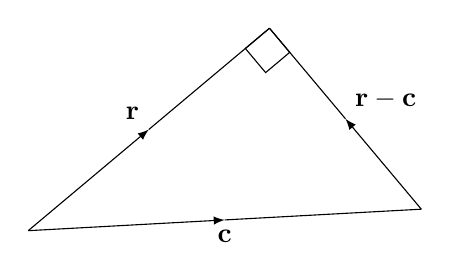
\begin{tikzpicture}[>=latex, rotate=130]
                % \tkzDefPoint(0,0){O}
                % \tkzDefPoint(1.732,0){R}
                % \tkzDefPoint(-30:2){C}
                \tkzDefPoint(0,4){O}
                \tkzDefPoint(0,0){R}
                \tkzDefPoint(-3,0){C}

                \draw[draw=none] (O) -- coordinate[midway] (R') (R);
                \draw[draw=none] (O) -- coordinate[midway] (C') (C);
                \draw[draw=none] (C) -- coordinate[midway] (CR) (R);

                \draw (R') node[above left] {$\vec{r}$};
                \draw (C') node[below] {$\vec{c}$};
                \draw (CR) node[above right] {$\vec{r}-\vec{c}$};

                \draw[->] (O) -- (R');
                \draw (R') -- (R);

                \draw[->] (O) -- (C');
                \draw (C') -- (C);

                \draw[->] (C) -- (CR);
                \draw (CR) -- (R);

                \tkzMarkRightAngle[size=0.4](C,R,O)
            \end{tikzpicture}
        \end{center}

        Thus, $\vec{r}$ must be selected such that
        the angle formed by $\vec{r}$ and $\vec{r}-\vec{c}$ is a right angle.
        By a circle theorem, an angle subtended by the diameter is a right angle.
        Thus, $\vec{r}$ must be within the sphere with $\vec{c}$ as diameter,
        i.e. $\abs{\vec{r} - \vec{c}/2} = \abs{\vec{c}}/2$. Combining
        this with the fact that it must live in the plane through $\vec{c}$
        with normal vector $\vec{d}$, we get the intersection of a plane
        and a sphere, which is a circle.

        To be precise, the plane goes through $\vec{c}$
        and has normal vector $\unitvec{d}$, and the
        sphere goes through $\vec{c}$ and $\vec{0}$ and has those
        points form a diameter, i.e. center at $\vec{c}/2$.

        Up to now, we have only used the directional information in
        $\vec{r}\times\vec{d} = \vec{c}-\vec{r}$.
        Let's consider the magnitude. Let 
        $\lambda = \abs{\vec{r}\times\vec{d}} = \abs{\vec{c}-\vec{r}}$.

        We have that $\abs{\vec{c}-\vec{r}} = \lambda$
        forms another sphere, centered at $\vec{c}$,
        with radius $\lambda$. Since $\vec{r}$ also has to
        live within the plane, the intersection
        forms a circle centered at $\vec{c}$ with radius $\lambda$.
        
        For the cross product, we have that
        $\abs{\vec{r}\times\vec{d}}$ is the area of the parallelogram.
        A parallelogram's area is its base times its height,
        so if we let $\vec{d}$ be its base, it's clear that
        $\abs{\vec{r}\times\vec{d}} = \lambda$ forms
        an infinite cylinder with $\vec{d}$ as its axis,
        centered at $\vec{0}$. In other words, 
        \begin{align*}
            \abs{\vec{r}}\abs{\vec{d}}\sin\theta_{\vec{r}\vec{d}} &= \lambda\\
            \abs{\vec{r}}\sin\theta_{\vec{r}\vec{d}} &= \frac{\lambda}{\abs{\vec{d}}}
        \end{align*}
        Diagrammatically, we have
        \begin{center}
            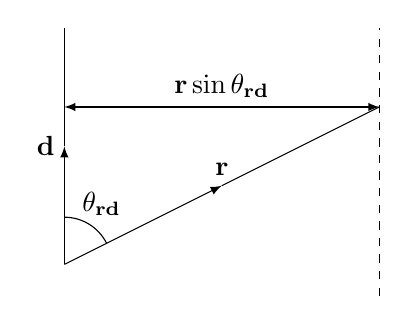
\begin{tikzpicture}[>=latex, scale=2]
                \tkzDefPoint(0,0){O}
                \tkzDefPoint(0,1.5){D}
                \tkzDefPoint(2,1){R}

                \draw[draw=none] (O) -- coordinate[midway] (D1) (D);
                \draw[draw=none] (O) -- coordinate[midway] (R1) (R);

                \draw[->] (O) -- (R1) node[above] {$\vec{r}$};
                \draw (R1) -- (R);
                \draw[->] (O) -- (D1) node[left] {$\vec{d}$};
                \draw (D1) -- (D);

                \tkzMarkAngle[size=0.3](R,O,D)
                \tkzLabelAngle[pos=0.45](R,O,D){$\theta_{\vec{r}\vec{d}}$}

                \draw[<->] (R) -- coordinate[midway] (RD) (R -| D);
                \draw (RD) node[above] {$\abs{\vec{r}}\sin\theta_{\vec{r}\vec{d}}$};

                \draw[dashed] (2,-0.2) -- (2,1.5);
            \end{tikzpicture}
        \end{center}
        So $\vec{r}$ can lie anywhere on the dashed line. Combined
        with radial symmetry around $\vec{d}$, we have the infinite cylinder.
        Since the infinite cylinder has axis $\vec{d}$, it is
        perpendicular to the plane. Thus, the intersection
        of the infinite cylinder with the plane is a circle with radius
        $\abs{\vec{r}}\sin\theta_{\vec{r}\vec{d}} = \lambda/\abs{\vec{d}}$,
        centered at the projection of $\vec{0}$ onto the plane.

        Thus any solution $\vec{r}$ must lie on both of
        the circles for some $\lambda$. Interestingly,
        the radius of the circles have a constant ratio of $\abs{\vec{d}}:1$,
        which means that so must the distances from $\vec{r}$ to the centre
        of each circle. Thus, the locus of possible $\vec{r}$ forms another circle,
        from the result from question 2. However, the equation of that
        circle is rather complicated, so this line of reasoning ends here.

        (ii)\\
        We have
        \begin{align*}
            \vec{r} + (\vec{r}\cdot\vec{a})\vec{b} &= \vec{c}\\
            ((\vec{r} - \vec{c} + \vec{c})\cdot\vec{a})\vec{b} &= \vec{c} - \vec{r}\\
            ((\vec{r} - \vec{c})\cdot\vec{a} + \vec{c}\cdot\vec{a})\vec{b}
            &= \vec{c} - \vec{r}\\
            ((\vec{c}\cdot\vec{a}) - (\vec{x}\cdot\vec{a}))\vec{b} &= \vec{x}
        \end{align*}
        We then have that $\vec{x} = \lambda \vec{b}$. Thus,
        \begin{align*}
            \lambda &= (\vec{c}\cdot\vec{a}) - \lambda(\vec{b}\cdot\vec{a})\\
            \lambda(1 + \vec{a}\cdot\vec{b}) &= \vec{a}\cdot\vec{c}\\
            \lambda &= \frac{\vec{a}\cdot\vec{c}}{1 + \vec{a}\cdot\vec{b}}\\
        \end{align*}
        So finally, we have
        \begin{align*}
        \vec{x} = \vec{c}-\vec{r} 
        &= \frac{\vec{a}\cdot\vec{c}}{1 + \vec{a}\cdot\vec{b}}\vec{b}\\
        \vec{r}
        &= \vec{c} - \frac{\vec{a}\cdot\vec{c}}{1 + \vec{a}\cdot\vec{b}}\vec{b}
        \end{align*}
    \end{answer}

    \begin{question}
        The vectors $\vec{e}_r, \vec{e}_\theta, \vec{e}_\phi$ are defined
        in terms of the standard basis vectors $\vec{i},\vec{j},\vec{k}$ by
        \begin{align*}
            \vec{e}_r &= \cos\phi\sin\theta\vec{i}+\sin\phi\sin\theta\vec{j}+\cos\theta\vec{k}\\
            \vec{e}_\theta &= \cos\phi\cos\theta\vec{i}+\sin\phi\cos\theta\vec{j}-\sin\theta\vec{k}\\
            \vec{e}_\phi &= -\sin\phi\vec{i}+\cos\phi\vec{j}
        \end{align*}
        where $\theta$ and $\phi$ are real numbers. Show,
        as effeciently as possible, that $\vec{e}_r, \vec{e}_\theta, \vec{e}_\phi$
        are an orthonormal right-handed set.
    \end{question}
    \begin{proof}
        Those equations heavily remind me of spherical coordinates.
        The labels $r,\theta,\phi$ are also clearly referencing spherical coordinates.
        It seems that $\vec{e}_\phi$ is the yaw vector,
        since it is simply a unit vector living in the $\vec{i}\vec{j}$-plane,
        with angle $\phi$. We have
        \[
            \abs{\vec{e}_\phi}^{2} = \sin^{2}\phi+\cos^{2}\phi = 1.
        \]
        Let $\vec{f}_\phi = \cos\phi\vec{i}+\sin\phi\vec{j}$.
        We claim $\vec{k},\vec{f}_\phi,\vec{e}_\phi$ forms a right-handed orthonormal basis.
        They are all clearly unit, and $\vec{e}_\phi$ and $\vec{f}_\phi$
        have no $\vec{k}$ component and are perpendicular to each other by
        $\vec{e}_\phi\cdot\vec{f}_\phi = -\sin\phi\cos\phi+\sin\phi\cos\phi = 0$.

        Finally, we consider right-handedness, through
        $\vec{k}\cdot(\vec{f}_\phi\times\vec{e}_\phi)$.
        Since $\vec{e}_\phi$ and $\vec{f}_\phi$ both live
        in the $\vec{i}\vec{j}$-plane, the cross product must be of the form $\lambda\vec{k}$.
        To be precise, 
        \begin{align*}
            \lambda 
            &= (\vec{f}_\phi)_1(\vec{e}_\phi)_2 - (\vec{f}_\phi)_2(\vec{e}_\phi)_1\\
            &= \cos\phi\cos\phi - (-\sin\phi\sin\phi) = 1
        \end{align*}
        Thus, $\vec{k}\cdot(\vec{f}_\phi\times\vec{e}_\phi) = \vec{k}\cdot\vec{k} = 1$,
        so it is right-handed.
        With this,
        \begin{align*}
            \vec{e}_r 
            &= \cos\phi\sin\theta\vec{i}+\sin\phi\sin\theta\vec{j}+\cos\theta\vec{k}\\
            &= \sin\theta(\cos\phi\vec{i}+\sin\phi\vec{j})+\cos\theta\vec{k}\\
            &= \cos\theta\vec{k}+\sin\theta\vec{f}_\phi\\
            \vec{e}_\theta 
            &= \cos\phi\cos\theta\vec{i}+\sin\phi\cos\theta\vec{j}-\sin\theta\vec{k}\\
            &= \cos\theta(\cos\phi\vec{i}+\sin\phi\vec{j})-\sin\theta\vec{k}\\
            &= -\sin\theta\vec{k}+\cos\theta\vec{f}_\phi
        \end{align*}
        Notice that under the new basis, $\vec{e}_\theta$ has
        the same coordinates as $\vec{e}_\phi$ had in the standard basis.
        Similarly, $\vec{e}_r$ has the same coordinates as $\vec{f}_\phi$.
        Thus, directly
        corresponding with $\vec{k},\vec{f}_\phi,\vec{e}_\phi$,
        we have that 
        $\vec{e}_\phi,\vec{e}_r,\vec{e}_\theta$
        form a right-handed orthonormal basis.

        Since $\vec{e}_\phi\cdot(\vec{e}_r\times\vec{e}_\theta)$ is invariant
        under cyclic permutation of $\vec{e}_\phi,\vec{e}_r,\vec{e}_\theta$,
        we know $\vec{e}_r,\vec{e}_\theta,\vec{e}_\phi$ are right-handed.
        Combined with the fact that
        orthonormality is invariant under permutation,
        we have that $\vec{e}_r,\vec{e}_\theta,\vec{e}_\phi$ are a right-handed
        orthonormal basis.
    \end{proof}
\end{document}
